\documentclass{amsart}
\usepackage{amssymb,amsmath,amsthm,mathrsfs,graphics,hyperref,stmaryrd,psfrag,arcs,xypic}
\usepackage[enableskew]{youngtab}
\numberwithin{equation}{section}
\raggedbottom
\oddsidemargin=0in
\evensidemargin=0in
\textwidth=6.5in
\textheight=8.8in
\topmargin=0.25in
\headheight=0in
\headsep=0.2in
\footskip=0in
\parskip=10bp
\parindent=0bp

\newcommand{\excise}[1]{}
\newcommand{\Latex}[1]{\textbackslash\texttt{#1}}

\newcommand{\bigpad}{\rule[-14mm]{0mm}{30mm}}
\newcommand{\smallpad}{\rule[-1.5mm]{0mm}{5mm}}
\newcommand{\pad}{\rule[-3mm]{0mm}{8mm}}
\newcommand{\padup}{\rule{0mm}{5mm}}
\newcommand{\paddown}{\rule[-3mm]{0mm}{2mm}}
\newcommand{\blank}{\rule{1.25in}{0.25mm}}
\newcommand{\commentout}[1]{}
\newcommand{\yell}[1]{\fbox{\rule[-1mm]{0mm}{4mm} \large\bf #1 }}
\newcommand{\bang}{$\bullet$\quad}
\newcommand{\indnt}{\phantom{.}\qquad}
\newcommand{\littleline}{\begin{center}\rule{4in}{0.5bp}\end{center}}

\newcommand{\includefigure}[3]{{
  \begin{center}
  \resizebox{#1}{#2}{\includegraphics{{figs/#3}}}
  \end{center}}}
\newcommand{\includefigurewithinmath}[3]{{
  \resizebox{#1}{#2}{\includegraphics{{figs/#3}}}}}

%\newcommand{\defterm}[1]{\underline{\textbf{#1}}}
\newcommand{\defterm}[1]{\textbf{#1}}

\DeclareMathOperator{\ch}{\mathbf{ch}}
\DeclareMathOperator{\colspace}{colspace}
\DeclareMathOperator{\corank}{corank}
\DeclareMathOperator{\CST}{CST}
\DeclareMathOperator{\deln}{del}
\DeclareMathOperator{\diag}{diag}
\DeclareMathOperator{\ess}{ess}
\DeclareMathOperator{\Gr}{Gr}
\DeclareMathOperator{\Hom}{Hom}
\DeclareMathOperator{\im}{im}
\DeclareMathOperator{\Irr}{Irr}
\DeclareMathOperator{\Ind}{Ind}
\DeclareMathOperator{\Int}{Int}
\DeclareMathOperator{\lcm}{lcm}
\DeclareMathOperator{\link}{lk}
\DeclareMathOperator{\nullity}{nullity}
\DeclareMathOperator{\nullspace}{nullspace}
\DeclareMathOperator{\Poin}{Poin}
\DeclareMathOperator{\proj}{proj}
\DeclareMathOperator{\rank}{rank}
\DeclareMathOperator{\Res}{Res}
\DeclareMathOperator{\Span}{span}
\DeclareMathOperator{\supp}{supp}
\DeclareMathOperator{\row}{row}
\DeclareMathOperator{\rowspace}{rowspace}
\DeclareMathOperator{\sh}{sh}
\DeclareMathOperator{\tr}{tr}
\DeclareMathOperator{\wt}{wt}

\newtheorem{theorem}{Theorem}[section]
\newtheorem{proposition}[theorem]{Proposition}
\newtheorem{lemma}[theorem]{Lemma}
\newtheorem{corollary}[theorem]{Corollary}
\theoremstyle{definition}
\newtheorem{definition}[theorem]{Definition}
\newtheorem{example}[theorem]{Example}
\newtheorem{remark}[theorem]{Remark}
\newtheorem{problem}[theorem]{Problem}


\newcommand{\cor}{{\bf Corollary: }}
\newcommand{\defn}{{\bf Definition: }}
\newcommand{\defns}{{\bf Definitions: }}
\newcommand{\exa}{{\bf Example: }}
\newcommand{\fact}{{\bf Fact: }}
\newcommand{\lem}{{\bf Lemma: }}
\newcommand{\notn}{{\bf Notation: }}
\newcommand{\obs}{{\bf Observation: }}
\newcommand{\note}{{\bf Note: }}
\newcommand{\prop}{{\bf Proposition: }}
\newcommand{\rmk}{{\bf Remark: }}
\newcommand{\thm}{{\bf Theorem: }}

\newcommand{\basecase}{\emph{Base case: }}
\newcommand{\indstep}{\emph{Inductive step: }}
\newcommand{\skpr}{\emph{Sketch of proof: }}

\newcommand{\0}{\emptyset}
\newcommand{\Alt}{\mathfrak{A}}
\newcommand{\Braid}{Br}
\newcommand{\CHI}{\chi^{\phantom{*}}}
\newcommand{\Cl}{C\ell}
\newcommand{\covers}{\gtrdot}
\newcommand{\coveredby}{\lessdot}
\newcommand{\dedge}[1]{\overrightarrow{{#1}}}
\newcommand{\dom}{\rhd}
\newcommand{\domeq}{\unrhd}
\newcommand{\domby}{\lhd}
\newcommand{\dombyeq}{\unlhd}
\newcommand{\Fspan}{\Ff\text{-span}}
\newcommand{\isom}{\cong}
\newcommand{\join}{\vee}
\renewcommand{\Join}{\bigvee}
\newcommand{\Laff}{L^{\text{aff}}}
\newcommand{\lin}[1]{\overleftrightarrow{{#1}}}
\newcommand{\meet}{\wedge}
\newcommand{\Meet}{\bigwedge}
\newcommand{\ov}[1]{\overline{{#1}}}
\newcommand{\partn}{\vdash}
\newcommand{\qqandqq}{\qquad\text{and}\qquad}
\newcommand{\qandq}{\quad\text{and}\quad}
\newcommand{\qand}{\quad\text{and}}
\newcommand{\qbin}[2]{{\begin{bmatrix}#1\\#2\end{bmatrix}_q}}
\newcommand{\sd}{\triangle} % symmetric difference
\newcommand{\simK}{\underset{K}{\sim}} % Knuth equivalence
\newcommand{\simJ}{\underset{J}{\sim}} % jeu de taquin equivalence
\newcommand{\sm}{\setminus}
\newcommand{\st}{~|~}
\newcommand{\soln}{\textit{Solution:\ }}
\newcommand{\Sym}{\mathfrak{S}}
\newcommand{\un}[1]{\underset{*}{#1}}
\newcommand{\unA}{\un{A}}
\newcommand{\unB}{\un{B}}
\newcommand{\unw}{\un{w}}
\newcommand{\unx}{\un{x}}
\newcommand{\uny}{\un{y}}
\newcommand{\unz}{\un{z}}
\newcommand{\x}{\times}

\renewcommand{\aa}{\mathbf{a}}
\newcommand{\bb}{\mathbf{b}}
\newcommand{\nn}{\mathbf{n}}
\newcommand{\pp}{\mathbf{p}}
\newcommand{\qq}{\mathbf{q}}
\newcommand{\xx}{\mathbf{x}}
\newcommand{\yy}{\mathbf{y}}
\newcommand{\zz}{\mathbf{z}}
 
\newcommand{\A}{\mathcal{A}}
\newcommand{\B}{\mathcal{B}}
\newcommand{\C}{\mathcal{C}}
\newcommand{\M}{\mathcal{M}}
\renewcommand{\P}{\mathcal{P}}

\newcommand{\BB}{\mathscr{B}}  %% use these for fancy script fonts -- requires mathrsfs package
\newcommand{\CC}{\mathscr{C}}
\newcommand{\FF}{\mathscr{F}}
\newcommand{\II}{\mathscr{I}}
\newcommand{\LL}{\mathscr{L}}
\newcommand{\PP}{\mathscr{P}}
\renewcommand{\SS}{\mathscr{S}}
\newcommand{\XX}{\mathscr{X}}

\newcommand{\TT}{\tilde{T}}

\newcommand{\Aa}{\mathbb{A}}
\newcommand{\Cc}{\mathbb{C}}
\newcommand{\Ff}{\mathbb{F}}
\newcommand{\Nn}{\mathbb{N}}
\newcommand{\Pp}{\mathbb{P}}
\newcommand{\Qq}{\mathbb{Q}}
\newcommand{\Rr}{\mathbb{R}}
\newcommand{\Zz}{\mathbb{Z}}

\newcommand{\rhodef}{\rho^{\phantom{*}}_{{\rm def}}}
\newcommand{\rhotriv}{\rho^{\phantom{*}}_{{\rm triv}}}
\newcommand{\rhosign}{\rho^{\phantom{*}}_{{\rm sign}}}
\newcommand{\rhoreg}{\rho^{\phantom{*}}_{{\rm reg}}}
\newcommand{\chidef}{\chi^{\phantom{*}}_{{\rm def}}}
\newcommand{\chitriv}{\chi^{\phantom{*}}_{{\rm triv}}}
\newcommand{\chisign}{\chi^{\phantom{*}}_{{\rm sign}}}
\newcommand{\chireg}{\chi^{\phantom{*}}_{{\rm reg}}}
\newcommand{\scp}[2]{\left\langle #1,\:#2\right\rangle_G}
\newcommand{\scpH}[2]{\left\langle #1,\:#2\right\rangle_H}

\newcounter{probno}
\setcounter{probno}{0}
\newcounter{partno}
\setcounter{partno}{0}
%% versions that don't print the number of points
\newcommand{\prob}{
  \vskip10bp%
  \setcounter{partno}{0}%
  \addtocounter{probno}{1}%
  {\bf Problem~\#{\arabic{probno}}}\quad}
\newcommand{\probpart}{%\rule{0in}{0in}\\ \phantom{xxx}
  \addtocounter{partno}{1}%
  {\bf (\#\arabic{probno}\alph{partno})}\ \ }
\newcommand{\probcont}{%
  {\bf Problem~\#{\arabic{probno}}}~(\emph{continued})}
\newcommand{\probo}{
  \setcounter{partno}{0}%
  \addtocounter{probno}{1}%
  {\bf (\#\arabic{probno})}\ \ }
%% versions that do print the number of points
\newcommand{\Prob}[1]{
  \vskip10bp%
  \setcounter{partno}{0}%
  \addtocounter{probno}{1}%
  {\bf Problem~\#{\arabic{probno}}~[{#1}~pts]}\quad}
\newcommand{\Probpart}[1]{%\rule{0in}{0in}\\ \phantom{xxx}
  \addtocounter{partno}{1}%
  {\bf (\#\arabic{probno}\alph{partno})~[{#1}~pts]}\ \ }

%\renewcommand{\thefootnote}{\fnsymbol{footnote}}

\begin{document}
\thispagestyle{empty}

\textbf{Math 724, Fall 2017\\
Homework \#2\\
Deadline: Friday, September 15, 5:00pm}

\textbf{Instructions:} Typeset your solutions in LaTeX.  Email your solutions to Jeremy (jlmartin@ku.edu) as a PDF file named with your last name and the problem set number (e.g., {\tt Abel2.pdf}).  Collaboration is encouraged, but each student must write up his or her solutions independently and acknowledge all collaborators.

\medskip\hrule

\prob Bogart, Problem \#37.  (This is not supposed to be hard!)

\vfill\prob   Bogart, Problem \#56.

\vfill\prob   Bogart, Problem \#58.

\vfill\prob Bogart, Chapter 1 Supplementary Problem \#5.

\vfill\prob Bogart, Chapter 1 Supplementary Problem \#11.

\vfill\prob Call a set $S$ of numbers \emph{special} if no two pairs of numbers in $S$ have the same sum.  For example, $\{1,2,5,10,20\}$ is special, but $\{2,3,5,7,11,13\}$ is not special because $3+13=5+11$.

\probpart  Prove that if $S\subseteq\{1,2,\dots,100\}$ and $|S|\geq40$, then $S$ is not special.

\probpart  Can you tighten the bound of the previous problem?  In other words, find the smallest value $N$ for which your argument remains true upon replacing 40 with $N$.

\vfill\prob A \emph{plane tree} is a rooted tree in which the children of every vertex are ordered from oldest to youngest.  We conventionally draw plane trees by placing the root vertex at the top and placing the children of every vertex on a horizontal line below it, ordered left to right according to age.  This ordering matters; for example, the two trees below are considered to be different (on the left, the grandchild of the root is the child of its oldest child, while on the right, the grandchild is the child of its youngest child).

\begin{center}
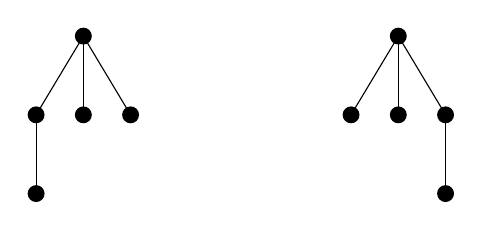
\begin{tikzpicture}
\draw[fill=black] (2,2) circle (0.1);
\foreach \x in {1.4,2,2.6} { \draw[fill=black] (\x,1) circle (0.1); \draw (2,2) -- (\x,1); }
\draw[fill=black] (1.4,0) circle (0.1); \draw (1.4,0) -- (1.4,1); 
\begin{scope}[shift={(4,0)}]
\draw[fill=black] (2,2) circle (0.1);
\foreach \x in {1.4,2,2.6} { \draw[fill=black] (\x,1) circle (0.1); \draw (2,2) -- (\x,1); }
\draw[fill=black] (2.6,0) circle (0.1); \draw (2.6,0) -- (2.6,1); 
\end{scope}
\end{tikzpicture}
\end{center}
Prove that the number of plane trees with $n+1$ vertices is the Catalan number $\frac{1}{n+1}\binom{2n}{n}$.  (Hint: Consider walking through the tree via ``depth-first search'': start at the root, and visit all the vertices, making sure to visit the children of each vertex in left to right order.  Stop when you return to the root; you should have crossed every edge twice.  Use this walk to construct a bijection between plane trees and Catalan paths.)

\vfill
{\bf Extra credit:} Let $P<Q$ be positive integers.  The students in a class are assigned to $P$ groups for in-class group work.  (Each group has at least one student in it.)  One day a substitute teacher comes in and rearranges the students into $Q$ groups.  Prove that at least $Q-P+1$ students end up in smaller groups.


\end{document}